% =========================================================
% main.tex
% Reusable Engineering Portfolio Report Template
% =========================================================
%
% NORMAL WORKFLOW
% ---------------
% 1. Edit public project metadata in setup/00_metadata.tex.
% 2. Replace the context, abstract, and objective in frontmatter/.
% 3. Register technical sections in content/00_report_body.tex.
% 4. Register appendices in appendices/00_appendices.tex.
% 5. Add analytical, simulation, and measurement records.
% 6. Compile with pdfLaTeX and Biber.
%
% This controller intentionally contains document assembly only.
% =========================================================

\documentclass[12pt,a4paper,oneside,openany]{report}

% 1. Public, user-editable project metadata
% =========================================================
% setup/00_metadata.tex
% Public, user-editable portfolio metadata
% =========================================================
%
% This is the first file to edit when starting a portfolio project.
% Keep plain-text PDF fields free of manual line breaks and commands.
% Escape LaTeX special characters when needed: & -> \&, % -> \%, _ -> \_.

% -----------------------------------------------------------------
% 1. Public project identity
% -----------------------------------------------------------------
\newcommand{\projecttitle}{Compact Sensor Array Design and Verification}
\newcommand{\projectsubtitle}{Analytical Development, Numerical Modeling, and Engineering Evidence}
\newcommand{\projectdomain}{Applied Electromagnetics and Embedded Sensing}
\newcommand{\projectshorttitle}{Compact Sensor Array}

% Formatted title for the cover.
\newcommand{\reporttitle}{%
    Compact Sensor Array Design\\[0.18cm]
    and Verification%
}

% Plain title for PDF metadata and accessibility.
\newcommand{\reporttitleplain}{Compact Sensor Array Design and Verification}

% -----------------------------------------------------------------
% 2. Public author identity
% -----------------------------------------------------------------
\newcommand{\authorname}{Author Name}
\newcommand{\authorrole}{Engineer and Technical Researcher}
\newcommand{\portfolioedition}{Independent Engineering Portfolio Project}
\newcommand{\publicationdate}{\today}

% Public links. Replace placeholders before publication.
\newcommand{\repositoryurl}{https://github.com/username/project-repository}
\newcommand{\linkedinurl}{https://www.linkedin.com/in/username}
\newcommand{\contactemail}{name@example.com}

% Set each switch to true or false.
\newif\ifshowauthorrole
\showauthorroletrue
\newif\ifshowrepository
\showrepositorytrue
\newif\ifshowlinkedin
\showlinkedinfalse
\newif\ifshowcontactemail
\showcontactemailfalse

% -----------------------------------------------------------------
% 3. Optional public logo or project mark
% -----------------------------------------------------------------
\newif\ifshowprojectlogo
\showprojectlogofalse
\newcommand{\projectlogo}{figures/project-logo-placeholder.png}
\newcommand{\projectlogowidth}{4.6cm}

% -----------------------------------------------------------------
% 4. Portfolio context and evidence declarations
% -----------------------------------------------------------------
\newcommand{\projectorigin}{%
This public edition was prepared from an independently completed engineering project.
Replace this sentence with a concise, factual description of the project origin.}

\newcommand{\publiceditionnote}{%
Administrative, grading, student-identification, and institutional material has
been removed. The public edition focuses on technical decisions, evidence, limitations,
and reproducibility.}

\newcommand{\analyticalevidence}{%
Closed-form calculations, governing equations, design rules, and independent scripts.}

\newcommand{\simulatedevidence}{%
Numerical model construction, solver settings, parameter sweeps, and exported results.}

\newcommand{\measuredevidence}{%
No fabricated prototype or measurement campaign is claimed in this example template.}

\newcommand{\numericalscope}{%
Replace this paragraph with solver, mesh, boundary, material, convergence, and software
limitations that materially affect interpretation of the reported results.}

\newcommand{\affiliationdisclaimer}{%
This document is an independent portfolio artifact and does not imply endorsement by an
employer, university, instructor, customer, software vendor, or standards organization.}

% -----------------------------------------------------------------
% 5. Running headers and PDF properties
% -----------------------------------------------------------------
\newcommand{\headerleft}{Engineering Portfolio}
\newcommand{\headerright}{\projectshorttitle}
\newcommand{\pdfsubjecttext}{\projectdomain}
\newcommand{\pdfkeywordstext}{engineering portfolio, analytical design, numerical simulation, verification, reproducibility, technical documentation}


% 2. Shared portfolio-report setup
% =========================================================
% setup/01_packages.tex
% Core packages for the portfolio report
% =========================================================
\usepackage[utf8]{inputenc}
\usepackage[T1]{fontenc}
\usepackage[english]{babel}
\usepackage{lmodern}
\usepackage{microtype}

\usepackage{amsmath,amssymb,amsfonts,amsthm,mathtools,bm}
\usepackage{graphicx}
\usepackage{float}
\usepackage{xcolor}
\usepackage{booktabs}
\usepackage{tabularx}
\usepackage{longtable}
\usepackage{array}
\usepackage{multirow}
\usepackage{enumitem}
\usepackage{geometry}
\usepackage{fancyhdr}
\usepackage{caption}
\usepackage{subcaption}
\usepackage{titlesec}
\usepackage{siunitx}
\usepackage{textcomp}
\usepackage{upquote}
\usepackage{listings}
\usepackage{tikz}
\usetikzlibrary{arrows.meta,positioning,shapes.geometric,fit,calc}
\usepackage[most]{tcolorbox}
\usepackage{csquotes}
\usepackage[
    backend=bibtex,
    style=ieee,
    sorting=none,
    doi=true,
    isbn=false
]{biblatex}
\usepackage[
    colorlinks=true,
    linkcolor=blue!55!black,
    citecolor=red!55!black,
    urlcolor=cyan!45!black,
    breaklinks=true
]{hyperref}
\usepackage[nottoc]{tocbibind}

\sisetup{detect-all,per-mode=symbol}

% =========================================================
% setup/02_layout.tex
% Page geometry, headers, captions, and spacing
% =========================================================
\geometry{
    a4paper,
    top=2.4cm,
    bottom=2.5cm,
    left=2.8cm,
    right=2.5cm,
    headheight=16pt,
    includeheadfoot
}

\pagestyle{fancy}
\fancyhf{}
\fancyhead[L]{\small\slshape\nouppercase{\headerleft}}
\fancyhead[R]{\small\slshape\nouppercase{\headerright}}
\fancyfoot[C]{\thepage}
\renewcommand{\headrulewidth}{0.4pt}
\renewcommand{\footrulewidth}{0pt}

\fancypagestyle{plain}{%
    \fancyhf{}%
    \fancyhead[L]{\small\slshape\nouppercase{\headerleft}}%
    \fancyhead[R]{\small\slshape\nouppercase{\headerright}}%
    \fancyfoot[C]{\thepage}%
    \renewcommand{\headrulewidth}{0.4pt}%
    \renewcommand{\footrulewidth}{0pt}%
}

\fancypagestyle{titlepage}{%
    \fancyhf{}%
    \renewcommand{\headrulewidth}{0pt}%
    \renewcommand{\footrulewidth}{0pt}%
}

\captionsetup{margin=10pt,font=small,labelfont=bf}
\setlength{\parindent}{0pt}
\setlength{\parskip}{0.62em}
\allowdisplaybreaks
\setcounter{tocdepth}{3}
\setcounter{secnumdepth}{3}
\renewcommand{\listfigurename}{List of Figures}
\renewcommand{\listtablename}{List of Tables}

% =========================================================
% setup/03_math_macros.tex
% Reusable engineering notation
% =========================================================
\newcommand{\R}{\mathbb{R}}
\newcommand{\C}{\mathbb{C}}
\newcommand{\E}{\mathbb{E}}
\newcommand{\mat}[1]{\mathbf{#1}}
\renewcommand{\vec}[1]{\bm{#1}}
\newcommand{\T}{^{\mathsf{T}}}
\newcommand{\He}{^{\mathsf{H}}}
\newcommand{\dd}{\,\mathrm{d}}
\DeclareMathOperator{\diag}{diag}
\DeclareMathOperator{\tr}{tr}
\DeclareMathOperator{\rank}{rank}
\DeclarePairedDelimiter{\norm}{\lVert}{\rVert}
\DeclarePairedDelimiter{\abs}{\lvert}{\rvert}
\DeclareMathOperator*{\argmax}{arg\,max}
\DeclareMathOperator*{\argmin}{arg\,min}

% =========================================================
% setup/04_code_styles.tex
% Central code and console styles
% =========================================================
\definecolor{CodeBackground}{RGB}{244,248,252}
\definecolor{CodeFrame}{RGB}{116,145,170}
\definecolor{CodeKeyword}{RGB}{0,65,155}
\definecolor{CodeComment}{RGB}{0,120,65}
\definecolor{CodeString}{RGB}{160,30,30}
\definecolor{CodeNumber}{RGB}{105,105,105}

\lstdefinestyle{PortfolioPython}{
    language=Python,
    backgroundcolor=\color{CodeBackground},
    basicstyle=\ttfamily\footnotesize,
    keywordstyle=\color{CodeKeyword}\bfseries,
    commentstyle=\color{CodeComment}\itshape,
    stringstyle=\color{CodeString},
    numbers=left,
    numberstyle=\tiny\color{CodeNumber},
    numbersep=8pt,
    frame=single,
    rulecolor=\color{CodeFrame},
    framerule=0.5pt,
    framesep=6pt,
    showstringspaces=false,
    keepspaces=true,
    columns=fullflexible,
    upquote=true,
    tabsize=4,
    breaklines=true,
    breakatwhitespace=true,
    captionpos=b
}

\lstdefinestyle{PortfolioConsole}{
    backgroundcolor=\color{black!4},
    basicstyle=\ttfamily\footnotesize,
    numbers=none,
    frame=single,
    rulecolor=\color{black!35},
    showstringspaces=false,
    keepspaces=true,
    columns=fullflexible,
    breaklines=true,
    captionpos=b
}

% =========================================================
% setup/05_environments.tex
% Evidence, decision, limitation, and claim environments
% =========================================================
\definecolor{AnalyticalColor}{RGB}{0,88,150}
\definecolor{SimulatedColor}{RGB}{112,67,150}
\definecolor{MeasuredColor}{RGB}{25,125,70}
\definecolor{LimitationColor}{RGB}{170,85,0}
\definecolor{DecisionColor}{RGB}{65,65,65}

\newtcolorbox{analyticalevidencebox}[1][]{
    enhanced,breakable,colback=AnalyticalColor!5,colframe=AnalyticalColor,
    title={Analytical Evidence},fonttitle=\bfseries,#1
}
\newtcolorbox{simulatedevidencebox}[1][]{
    enhanced,breakable,colback=SimulatedColor!5,colframe=SimulatedColor,
    title={Simulated Evidence},fonttitle=\bfseries,#1
}
\newtcolorbox{measuredevidencebox}[1][]{
    enhanced,breakable,colback=MeasuredColor!5,colframe=MeasuredColor,
    title={Measured Evidence},fonttitle=\bfseries,#1
}
\newtcolorbox{limitationbox}[1][]{
    enhanced,breakable,colback=LimitationColor!7,colframe=LimitationColor,
    title={Limitation or Qualification},fonttitle=\bfseries,#1
}
\newtcolorbox{engineeringdecision}[1][]{
    enhanced,breakable,colback=DecisionColor!5,colframe=DecisionColor,
    title={Engineering Decision},fonttitle=\bfseries,#1
}

\newcommand{\evidencetag}[1]{%
    \tcbox[on line,boxrule=0.5pt,arc=2pt,left=3pt,right=3pt,top=1pt,bottom=1pt,
    colback=black!3,colframe=black!45]{\scriptsize\bfseries #1}%
}
\newcommand{\AnalyticalTag}{\evidencetag{ANALYTICAL}}
\newcommand{\SimulatedTag}{\evidencetag{SIMULATED}}
\newcommand{\MeasuredTag}{\evidencetag{MEASURED}}
\newcommand{\QualifiedTag}{\evidencetag{QUALIFIED}}

% Safe inclusion helper: missing figures produce a visible diagnostic box.
\newcommand{\maybeincludegraphics}[2][]{%
  \IfFileExists{#2}{%
    \includegraphics[#1]{#2}%
  }{%
    \fbox{%
      \begin{minipage}[c][0.20\textheight][c]{0.90\textwidth}
        \centering\small Missing figure file:\par\scriptsize\nolinkurl{#2}
      \end{minipage}%
    }%
  }%
}

% Consistent verification-matrix row command.
\newcommand{\VerificationRow}[5]{%
    #1 & #2 & #3 & #4 & #5\\
    \addlinespace[2pt]
}
% =========================================================
% setup/06_theme.tex
% Portfolio-report visual hierarchy
% =========================================================
\definecolor{ChapterColor}{RGB}{112,0,30}
\definecolor{SectionColor}{RGB}{0,55,105}
\definecolor{SubsectionColor}{RGB}{65,65,65}

\titleformat{\chapter}[display]
  {\normalfont\huge\bfseries\color{ChapterColor}}
  {\chaptertitlename\ \thechapter}
  {16pt}
  {\Huge}

\titleformat{\section}
  {\normalfont\Large\bfseries\color{SectionColor}}
  {\thesection}{0.8em}{}

\titleformat{\subsection}
  {\normalfont\large\bfseries\color{SubsectionColor}}
  {\thesubsection}{0.8em}{}


% 3. PDF metadata
\hypersetup{
    pdftitle={\reporttitleplain},
    pdfauthor={\authorname},
    pdfsubject={\pdfsubjecttext},
    pdfkeywords={\pdfkeywordstext}
}

% 4. Bibliography database
\addbibresource{references.bib}

\begin{document}

% Public cover: no academic identifiers or institutional branding by default.
\hypersetup{pageanchor=false}
% =========================================================
% frontmatter/titlepage.tex
% Public portfolio cover; normally edit metadata, not this layout.
% =========================================================
\begin{titlepage}
    \thispagestyle{titlepage}
    \centering

    \vspace*{1.2cm}

    \ifshowprojectlogo
        \IfFileExists{\projectlogo}{%
            \includegraphics[width=\projectlogowidth]{\projectlogo}\par
        }{%
            \fbox{\parbox[c][2.2cm][c]{0.72\textwidth}{\centering
            Project logo enabled but not found:\\[0.15cm]
            \texttt{\projectlogo}}}\par
        }
        \vspace{0.8cm}
    \fi

    \rule{\textwidth}{0.7pt}\par
    \vspace{0.65cm}

    {\Huge\bfseries\reporttitle\par}
    \vspace{0.45cm}
    {\Large\projectsubtitle\par}
    \vspace{0.28cm}
    {\large\color{SectionColor}\projectdomain\par}

    \vspace{0.65cm}
    \rule{\textwidth}{0.7pt}\par

    \vfill

    {\Large\bfseries\authorname\par}
    \ifshowauthorrole
        \vspace{0.18cm}
        {\large\authorrole\par}
    \fi

    \vspace{0.42cm}
    {\large\portfolioedition\par}

    \vfill

    \begin{minipage}{0.88\textwidth}
    \centering\small
    \ifshowrepository
        \textbf{Repository:} \url{\repositoryurl}\par
    \fi
    \ifshowlinkedin
        \textbf{LinkedIn:} \url{\linkedinurl}\par
    \fi
    \ifshowcontactemail
        \textbf{Contact:} \href{mailto:\contactemail}{\contactemail}\par
    \fi
    \end{minipage}

    \vspace{0.65cm}
    {\large\publicationdate\par}
\end{titlepage}

\hypersetup{pageanchor=true}

% Portfolio front matter uses Roman page numbering.
\clearpage
\pagenumbering{roman}
\setcounter{page}{1}
\pagestyle{fancy}

% =========================================================
% frontmatter/portfolio_context.tex
% Public context, evidence classes, and disclaimer
% =========================================================
\chapter*{Portfolio Context and Evidence}
\addcontentsline{toc}{chapter}{Portfolio Context and Evidence}

\textbf{Project origin.} \projectorigin

\textbf{Public portfolio edition.} \publiceditionnote

\begin{analyticalevidencebox}
\analyticalevidence
\end{analyticalevidencebox}

\begin{simulatedevidencebox}
\simulatedevidence
\end{simulatedevidencebox}

\begin{measuredevidencebox}
\measuredevidence
\end{measuredevidencebox}

\begin{limitationbox}
\numericalscope
\end{limitationbox}

\textbf{Affiliation disclaimer.} \affiliationdisclaimer

\vfill
\begin{center}
\textit{Prepared as a public engineering portfolio artifact.}
\end{center}

\clearpage
\chapter*{Abstract}
\addcontentsline{toc}{chapter}{Abstract}

This template demonstrates how to convert a completed engineering project into a
public, evidence-based portfolio report. The example narrative separates analytical
work, numerical simulation, and measured evidence; records assumptions and
limitations; and connects each public claim to a reproducible source. Replace this
sample abstract with a concise statement of the engineering problem, method,
principal verified results, and practical significance. Avoid unqualified performance
claims and clearly distinguish simulated behavior from measured hardware performance.

\clearpage
\chapter*{Project Objective}
\addcontentsline{toc}{chapter}{Project Objective}

The objective of this portfolio report is to document a complete engineering workflow
from problem definition through analytical design, model construction, numerical or
experimental verification, interpretation, and public claim control. The final report
should allow a technically competent reviewer to understand what was designed, why
specific decisions were made, what evidence supports the conclusions, and which
limitations remain unresolved.

\begin{engineeringdecision}
A portfolio report is not merely a shortened academic submission. It is a public
engineering artifact organized around judgment, evidence, reproducibility, and honest
qualification of uncertainty.
\end{engineeringdecision}


\clearpage
\tableofcontents
\clearpage
\listoffigures
\clearpage
\listoftables

% Main engineering narrative uses Arabic page numbering.
\clearpage
\pagenumbering{arabic}
\setcounter{page}{1}
\pagestyle{fancy}
% Central body menu: add, remove, or reorder chapters here.
\chapter{Project Overview}

\section{Engineering problem}
State the practical engineering problem in terms a hiring manager, customer, or
technical reviewer can evaluate. Identify the operating environment, performance
objective, constraints, and consequences of failure. Replace generic phrases such as
``optimize the system'' with measurable engineering targets.

\section{System context}
Figure~\ref{fig:portfolio-workflow} shows the recommended evidence flow for a public
engineering project. The report begins with requirements, proceeds through analytical
and numerical work, and ends with controlled public claims.

\begin{figure}[H]
\centering
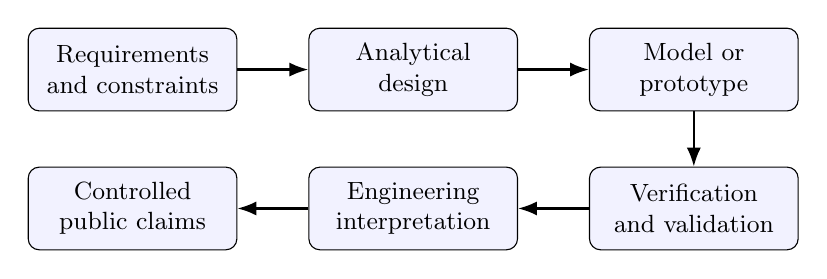
\begin{tikzpicture}[
  node distance=7mm and 9mm,
  box/.style={draw,rounded corners,minimum width=2.65cm,minimum height=1.05cm,
              align=center,fill=blue!5,font=\small},
  arr/.style={-{Latex[length=2.4mm]},thick}
]
\node[box] (req) {Requirements\\and constraints};
\node[box,right=of req] (ana) {Analytical\\design};
\node[box,right=of ana] (model) {Model or\\prototype};
\node[box,below=of model] (verify) {Verification\\and validation};
\node[box,left=of verify] (judge) {Engineering\\interpretation};
\node[box,left=of judge] (claim) {Controlled\\public claims};
\draw[arr] (req) -- (ana);
\draw[arr] (ana) -- (model);
\draw[arr] (model) -- (verify);
\draw[arr] (verify) -- (judge);
\draw[arr] (judge) -- (claim);
\end{tikzpicture}
\caption{Recommended evidence flow for an engineering portfolio project.}
\label{fig:portfolio-workflow}
\end{figure}

\section{Portfolio value}
Explain what this project demonstrates beyond software operation. Examples include
requirements translation, model credibility, trade-space reasoning, numerical
reliability, root-cause analysis, design iteration, verification discipline, and
technical communication.

\chapter{Engineering Scope and Evidence}

\section{Scope boundaries}
Define what is included and excluded. A strong scope statement prevents the public
report from implying fabrication, certification, field validation, or production
readiness that was not actually achieved.

\begin{table}[H]
\centering
\caption{Example scope boundary table.}
\label{tab:scope}
\begin{tabularx}{\textwidth}{>{\bfseries}p{0.22\textwidth}XX}
\toprule
Area & Included & Excluded or deferred \\
\midrule
Analytical work & Governing equations, first-order sizing, sensitivity checks & Formal uncertainty propagation \\
Numerical work & Baseline model, parameter sweep, selected convergence checks & Full certification-grade validation \\
Hardware & Interface and test concept & Fabricated prototype and chamber measurements \\
Public release & Verified plots, scripts, assumptions, limitations & Proprietary files and institution-specific administration \\
\bottomrule
\end{tabularx}
\end{table}

\section{Evidence taxonomy}
Use evidence labels consistently throughout the report:

\begin{itemize}[leftmargin=2em]
\item \AnalyticalTag\ results derived from equations, calculations, or independent scripts;
\item \SimulatedTag\ results exported from a numerical model or digital twin;
\item \MeasuredTag\ results obtained from physical instrumentation or test equipment;
\item \QualifiedTag\ claims that remain dependent on stated assumptions or incomplete validation.
\end{itemize}

\section{Deliverables}
List the public artifacts that allow a reviewer to reproduce or audit the work: source
report, code, console output, model screenshots, run manifest, parameter tables,
verification matrix, and selected native project files when licensing and size permit.

\chapter{Theory and Analytical Design}

\section{Governing model}
Introduce only the theory needed to justify engineering choices. For antenna and array projects, canonical references such as Stutzman and Thiele provide a disciplined starting point for notation and first-order design relationships~\cite{stutzman2012}. Define variables,
assumptions, coordinate systems, and validity limits. For an illustrative normalized
array or sensing problem, a generic response may be written as
\begin{equation}
H(\theta)=\sum_{n=0}^{N-1} w_n e^{j n \psi(\theta)},
\label{eq:generic-response}
\end{equation}
where $w_n$ represents a complex weighting coefficient and $\psi(\theta)$ represents
the progressive phase associated with geometry and excitation.

\section{First-order design calculation}
Show the calculation chain that converts requirements into initial dimensions or
parameters. The purpose is not to reproduce a textbook chapter; it is to establish a
traceable starting point for modeling and optimization.

\begin{analyticalevidencebox}
The example script in Appendix~\ref{app:analytical-verification} calculates a normalized
wavelength, nominal spacing, and progressive phase. Replace it with the project's real
verification script and retain its console output under \texttt{verification\_records/}.
\end{analyticalevidencebox}

\section{Assumptions and validity}
Record assumptions before presenting results. Typical examples include linearity,
steady-state operation, homogeneous materials, ideal source behavior, negligible
connector effects, limited temperature range, or simplified boundary conditions.

\chapter{Model and Simulation Method}

\section{Model construction}
Describe geometry, material properties, excitations, ports, boundary conditions,
monitors, mesh controls, solver type, stopping criteria, and post-processing. A second
engineer should be able to reconstruct the model from the information presented here
and in the simulation record.

\section{Parameter control}
Maintain a single source of truth for design parameters. Table~\ref{tab:parameters}
illustrates a compact public parameter record.

\begin{table}[H]
\centering
\caption{Example public parameter record.}
\label{tab:parameters}
\begin{tabular}{llll}
\toprule
Parameter & Symbol & Example value & Evidence source \\
\midrule
Reference frequency & $f_0$ & \SI{2.50}{\giga\hertz} & Requirement \\
Normalized wavelength & $\lambda_0$ & \SI{119.9}{\milli\meter} & Analytical script \\
Nominal spacing & $d$ & $0.5\lambda_0$ & Analytical design \\
Relative phase & $\alpha$ & \ang{90} & Steering case \\
\bottomrule
\end{tabular}
\end{table}

\section{Run manifest}
Record each meaningful numerical run with a stable identifier, model revision, solver,
mesh or discretization setting, changed parameter, completion status, and exported
artifacts. The starter file \texttt{simulation\_records/run\_manifest.csv} provides a
machine-readable structure.

\begin{simulatedevidencebox}
A screenshot alone is not a complete simulation record. Pair every published plot with
a run identifier and enough configuration information to reconstruct its origin.
\end{simulatedevidencebox}

\chapter{Results and Verification}

\section{Result presentation}
Present the minimum set of figures and tables needed to support the engineering
conclusion. Each caption should identify the evidence class, operating condition, and
relevant run or test identifier.

\begin{table}[H]
\centering
\caption{Example comparison of analytical and numerical evidence.}
\label{tab:comparison}
\begin{tabularx}{\textwidth}{>{\bfseries}p{0.28\textwidth}XXX}
\toprule
Metric & Analytical & Simulated & Interpretation \\
\midrule
Characteristic frequency & Requirement-derived & Solver-extracted & Agreement must be quantified \\
Primary response & Idealized model & Full numerical model & Differences require physical explanation \\
Efficiency or loss & Simplified estimate & Material and solver dependent & State model fidelity \\
Steering or control & Closed-form prediction & Post-processed result & Report scan loss and asymmetry \\
\bottomrule
\end{tabularx}
\end{table}

\section{Verification checks}
Verification asks whether the equations, scripts, model, and post-processing were
implemented correctly. Useful checks include unit tests, hand calculations,
independent scripts, reciprocity, symmetry, conservation, limiting cases, and
comparison with canonical results.

\section{Validation status}
Validation asks whether the model represents physical reality adequately for the
intended use. Explicitly distinguish model verification from experimental validation.

\begin{measuredevidencebox}
This starter report claims no measured evidence. Replace this box only after a real
prototype, calibrated setup, test procedure, uncertainty statement, and traceable data
record exist.
\end{measuredevidencebox}

\chapter{Engineering Discussion}

\section{Interpretation rather than description}
Do not merely restate that a curve moved or a field pattern changed. Explain the
physical or algorithmic mechanism, identify the controlling parameter, and connect the
result to requirements and design risk.

\section{Trade-offs}
Engineering portfolios become credible when trade-offs are explicit. Discuss competing
objectives such as bandwidth versus size, accuracy versus runtime, isolation versus
spacing, latency versus resource use, robustness versus complexity, and maintainability
versus optimization.

\section{Numerical reliability and limitations}
Document mesh or discretization adequacy, boundary sensitivity, solver tolerance,
material fidelity, numerical noise, anomalous behavior, and convergence evidence. Verification and validation should be treated as distinct technical activities rather than interchangeable labels~\cite{oberkampf2010,asmev20}.

\begin{limitationbox}
A visually smooth plot is not proof of numerical reliability. Non-monotonic or
unexpected behavior should trigger mesh, boundary, solver, or implementation checks.
When those checks are not feasible, state the limitation directly and narrow the claim.
\end{limitationbox}

\section{Industrial relevance}
Translate the technical result into a design, integration, manufacturing, maintenance,
safety, cost, or deployment consequence. This section should demonstrate engineering
judgment rather than marketing language.

\chapter{Engineering Verification Matrix}

The verification matrix is the claim-control center of the public report. Every major
claim should identify its evidence class, source, and limitation. Replace the sample
rows with project-specific entries before publication.

\begingroup
\small
\renewcommand{\arraystretch}{1.25}
\setlength{\tabcolsep}{4pt}

\begin{longtable}{
    @{}
    >{\centering\arraybackslash}p{0.055\textwidth}
    >{\raggedright\arraybackslash}p{0.27\textwidth}
    >{\raggedright\arraybackslash}p{0.13\textwidth}
    >{\raggedright\arraybackslash}p{0.24\textwidth}
    >{\raggedright\arraybackslash}p{0.20\textwidth}
    @{}
}

\caption{Engineering verification matrix.}
\label{tab:verification-matrix}
\\

\toprule
\textbf{ID}
&
\textbf{Public claim}
&
\textbf{Evidence class}
&
\textbf{Evidence location}
&
\textbf{Limitation or qualification}
\\
\midrule
\endfirsthead

\toprule
\textbf{ID}
&
\textbf{Public claim}
&
\textbf{Evidence class}
&
\textbf{Evidence location}
&
\textbf{Limitation or qualification}
\\
\midrule
\endhead

\midrule
\multicolumn{5}{r}{\small Continued on next page}
\\
\endfoot

\bottomrule
\endlastfoot

\VerificationRow
    {V1}
    {Initial dimensions or parameters were calculated independently.}
    {Analytical}
    {Equation~\eqref{eq:generic-response};
     Appendix~\ref{app:analytical-verification}}
    {Depends on stated first-order assumptions.}

\VerificationRow
    {V2}
    {The numerical model reproduces the documented baseline configuration.}
    {Simulated}
    {Model-method chapter; run manifest}
    {Requires project-specific solver and mesh records.}

\VerificationRow
    {V3}
    {The reported trend is physically interpreted and compared with the analytical expectation.}
    {Analytical + Simulated}
    {Results and discussion chapters}
    {Does not constitute experimental validation.}

\VerificationRow
    {V4}
    {No measured hardware performance is claimed in the starter document.}
    {Measured status}
    {Portfolio Context and Evidence}
    {Replace only after traceable physical testing.}

\end{longtable}
\endgroup

\chapter{Conclusion}

Summarize the verified engineering outcome, not the sequence of report sections. State
which requirements were met, which evidence supports that conclusion, what trade-offs
were accepted, and what remains unverified. Keep analytical, simulated, and measured
claims separate.

A strong final paragraph identifies the next technically defensible step, such as mesh
or boundary convergence, prototype fabrication, chamber measurement, hardware-in-the-
loop testing, environmental qualification, sensitivity analysis, or production design
review.



% Appendices contain reproducibility and run-record evidence.
\appendix
% Central appendix menu.
\chapter{Analytical Verification Script}
\label{app:analytical-verification}

This appendix demonstrates how to preserve an independent calculation inside the public
source package. Replace the starter script with the actual project calculation and
commit the corresponding console output.

\lstinputlisting[
    style=PortfolioPython,
    caption={Starter analytical verification script.},
    label={lst:analytical-script}
]{codes/analytical_verification.py}

\lstinputlisting[
    style=PortfolioConsole,
    caption={Recorded console output from the starter script.}
]{verification_records/analytical_results.txt}

\chapter{Simulation and Model Record}
\label{app:simulation-record}

For every published numerical result, retain a stable record containing the following:
\begin{itemize}[leftmargin=2em]
\item run identifier and model revision;
\item software and solver version;
\item geometry and material parameter set;
\item excitation, port, and boundary configuration;
\item mesh or discretization settings;
\item convergence or stopping criteria;
\item exported plots, tables, and raw data;
\item known warnings, simplifications, and failed checks.
\end{itemize}

\begin{table}[H]
\centering
\caption{Example simulation-run record.}
\begin{tabularx}{\textwidth}{>{\bfseries}p{0.24\textwidth}X}
\toprule
Field & Example entry \\
\midrule
Run ID & SIM-001 \\
Purpose & Baseline model before parameter sweep \\
Model revision & rev-A \\
Solver & Replace with solver and version \\
Discretization & Replace with cell count, mesh rule, or element order \\
Convergence & Replace with tolerance and achieved status \\
Artifacts & Plot names, raw exports, and screenshots \\
Limitations & Material, boundary, license, runtime, or memory constraints \\
\bottomrule
\end{tabularx}
\end{table}



\clearpage
\begingroup
\sloppy
\printbibliography[heading=bibintoc,title={References}]
\endgroup

\end{document}
